\documentclass[11pt,a4paper]{article}
\usepackage[utf8]{inputenc}
\usepackage{natbib}
\usepackage{authblk}
\usepackage{hyperref}
\usepackage{gensymb}
\usepackage{amsmath}

%\VignetteIndexEntry{User's guide to meteoland}
%\VignettePackage{meteoland}


\title{User's guide to meteoland (ver. 0.6.0)}
\author[1,2]{Miquel De Cáceres}
\affil[1]{Centre Tecnològic Forestal de Catalunya. Ctra. St. Llorenç de Morunys km 2, 25280, Solsona, Catalonia, Spain}
\affil[2]{CREAF, Cerdanyola del Vallès, 08193, Spain}

\usepackage{Sweave}
\begin{document}
\Sconcordance{concordance:Meteorology.tex:Meteorology.Rnw:%
1 16 1 1 0 7 1 1 5 32 1 1 2 14 0 1 2 1 1 1 2 14 0 1 2 5 1 1 %
2 1 0 1 1 4 0 1 2 4 1 1 2 13 0 1 2 1 1 1 2 16 0 1 2 32 1 1 %
2 40 0 1 2 8 1 1 2 16 0 1 2 10 1 1 24 7 1 1 9 1 2 35 1 2 2 %
2 1 1 4 1 2 36 1 2 2 2 1 1 4 1 2 19 1 2 2 2 1 2 2 19 1 2 2 %
19 1 1 5 4 1 1 18 1 2 9 1 1 37 1 2 28 1 1 51 1 2 2 1 1 34 1 %
2 2 1 1 34 1 2 17 1 1 56 1 2 28 1 2 2 2 1 2 2 18 1 1 27 1 2 %
2 1 1 7 6 1 1 12 1 2 16 1 1 26 1 2 28 1 2 2 2 1 2 2 67 1}


\maketitle
\tableofcontents

\newpage

\section{Introduction to the package}
\subsection{Purpose}
Reliable meteorological data are a basic requirement for hydrological and ecological studies at the landscape scale. Given the large spatial variation of meteorology over complex terrains, meteorological records from a single weather station are often not representative of entire landscapes. Studies made on multiple sites over a landscape require different meteorological series for each site; and other studies may require meteorological data series for all grid cells of a landscape, in a continuous way. In these cases, spatial correlation between the meteorology series of different sites or cells must be taken into account. For example, the sequence of days with rain of contiguous cells will normally be the same or very similar, even if precipitation amounts may differ. Finally, studies addressing the impacts of climate change on forests and landscapes require downscaling coarse-scale predictions  of global or regional climate models to the landscape scale. When downscaling predictions for several locations in a landscape, spatial correlation of predictions is also important.


With the aim to assist research of climatic impacts on forests, the R package \texttt{meteoland} provides utilities to estimate daily weather variables at any position in complex terrains:
\begin{enumerate}
\item{Spatial interpolation of daily weather records from meteorological stations. }
\item{Statistical correction of meteorological data series (e.g. from regional climate models).}
\end{enumerate}
Spatial interpolation is required when meteorology for the area and period of interest cannot be obtained from local measurements. The nearest weather station may not have data for the period of interest or it may be located too far away to be representative of the target area. Correcting the biases of a meteorological data series containing biases using a more accurate (i.e. local) meteorological series for a given reference period is necessary when the more accurate series does not cover the period of interest and the less accurate series does. The less accurate series may be at coarser scale, as with global/regional climate models or historical climate reanalysis. In this case one can speak of statistical downscaling. However, one may also correct the predictions of climate models using reanalysis data estimated at the same scale. 

\subsection{Data structures}
Package \texttt{meteoland} assists in the estimation of the following variables over lanscapes (units in parentheses):
\begin{itemize}
\item{\texttt{DOY}: Day of the year ([1-365]).}
\item{\texttt{MeanTemperature}: Mean daily temperature (in degrees Celsius).}
\item{\texttt{MinTemperature}: Minimum daily temperature (in degrees Celsius).}
\item{\texttt{MaxTemperature}: Maximum daily temperature (in degrees Celsius).}
\item{\texttt{Precipitation}: Daily precipitation (in mm of water).}
\item{\texttt{MeanRelativeHumidity}: Mean daily relative humidity (in percent).}
\item{\texttt{MinRelativeHumidity}: Minimum daily relative humidity (in percent).}
\item{\texttt{MaxRelativeHumidity}: Maximum daily relative humidity (in percent).}
\item{\texttt{Radiation}: Incoming radiation (in MJ/m2).}
\item{\texttt{WindSpeed}: Wind speed (in m/s).}
\item{\texttt{WindDirection}: Wind direction (in degrees from North).}
\item{\texttt{PET}: Potential evapo-transpiration (in mm of water).}
\end{itemize}

The package deals with two kinds of spatial structures: individual points and grids. The package includes four S4 spatial classes, which are defined as children of classes in package \texttt{sp}. 

\subsubsection{Topography}
Two classes are defined to represent the variation of topographic features (i.e., elevation, slope and aspect) over space:
\begin{itemize}
\item{\texttt{SpatialPointsTopography} extends \texttt{SpatialPointsDataFrame} and represents the topographic features of a set of points in a landscape.
\begin{Schunk}
\begin{Soutput}
Class "SpatialPointsTopography" [package "meteoland"]

Slots:
                                                                  
Name:         data  coords.nrs      coords        bbox proj4string
Class:  data.frame     numeric      matrix      matrix         CRS

Extends: 
Class "SpatialPointsDataFrame", directly
Class "SpatialPoints", by class "SpatialPointsDataFrame", distance 2
Class "Spatial", by class "SpatialPointsDataFrame", distance 3
\end{Soutput}
\end{Schunk}
}
\item{\texttt{SpatialGridTopography} extends \texttt{SpatialGridDataFrame} and represents the continuous variation of topographic features over all cells in a grid.
\begin{Schunk}
\begin{Soutput}
Class "SpatialGridTopography" [package "meteoland"]

Slots:
                                                          
Name:          data         grid         bbox  proj4string
Class:   data.frame GridTopology       matrix          CRS

Extends: 
Class "SpatialGridDataFrame", directly
Class "SpatialGrid", by class "SpatialGridDataFrame", distance 2
Class "Spatial", by class "SpatialGridDataFrame", distance 3
\end{Soutput}
\end{Schunk}
}
\end{itemize}
Although they have the same slots as their parent S4 classes, data frames in \texttt{SpatialPointsTopography} and \texttt{SpatialGridTopography} objects have only three variables: `\textbf{elevation}' (in meters), `\textbf{slope}' (in degrees) and `\textbf{aspect}' (in degrees from North).

\subsubsection{Meteorology}
Analogously to topography, two spatial classes are used to represent the variation of daily meteorology over space:
\begin{itemize}
\item{\texttt{SpatialPointsMeteorology} extends \texttt{SpatialPoints} and represents daily meteorology series for a set of points in a landscape.
\begin{Schunk}
\begin{Soutput}
Class "SpatialPointsMeteorology" [package "meteoland"]

Slots:
                                                                  
Name:        dates        data      coords        bbox proj4string
Class:        Date      vector      matrix      matrix         CRS

Extends: 
Class "SpatialPoints", directly
Class "Spatial", by class "SpatialPoints", distance 2
\end{Soutput}
\end{Schunk}
}
\item{\texttt{SpatialGridMeteorology} extends \texttt{SpatialGrid} and represents the continuous variation of daily meteorology across a grid of cells.
\begin{Schunk}
\begin{Soutput}
Class "SpatialGridMeteorology" [package "meteoland"]

Slots:
                                                          
Name:         dates         data         grid         bbox
Class:         Date       vector GridTopology       matrix
                   
Name:   proj4string
Class:          CRS

Extends: 
Class "SpatialGrid", directly
Class "Spatial", by class "SpatialGrid", distance 2
\end{Soutput}
\end{Schunk}
}
\end{itemize}
In addition to their corresponding inherited slots, \texttt{SpatialPointsMeteorology} and \texttt{SpatialGridMeteorology} have two additional slots: `\texttt{dates}' (a vector of days specifying a time period), and `\texttt{data}' (a vector of data frames with the meteorological data).
Although both classes have a `\texttt{data}' slot containing data frames, meteorological data is in different form in each class. In objects of \texttt{SpatialPointsMeteorology}, there is one data frame for each point where variables are in columns and dates are in rows. In objects of \texttt{SpatialGridMeteorology}, each data frame describes the meteorology over the grid for a single day. In this case, the data frame has grid cells in rows and variables in columns.

The package provides two functions to extract/reshape meteorological data from these structures:
\begin{itemize}
\item{Function \texttt{extractgridpoints()} extracts the meteorology of particular points in a grid (it returns an object of \texttt{SpatialPointsMeteorology}).}
\item{Function \texttt{extractpointdates()} extracts the meteorology of a set of dates from an object of class \texttt{SpatialPointsMeteorology}. It returns one data frame for each date, with points in rows and meteorology variables in columns.}
\end{itemize}

\subsection{Reading and writing meteorological data}
\subsubsection{Point meteorology}
Objects of class \texttt{SpatialPointsMeteorology} are stored in the disk using one \textbf{ascii} data file for each of their spatial points. Package \texttt{meteoland} provides four input/output functions for point meteorology:
\begin{itemize}
\item{Function \texttt{readmeteorologypoint()} reads the meteorological data stored in one \textbf{ascii} data file and returns a data frame.}
\item{Function \texttt{writemeteorologypoint()} writes the meteorological data of a single point as an \textbf{ascii} file in the file system.}
\item{Function \texttt{readmeteorologypointfiles()} reads several \textbf{ascii} files and returns an object of class \texttt{SpatialPointsMeteorology}.}
\item{Functions \texttt{writemeteorologypointfiles()} writes several \textbf{ascii} files in the disk, one per spatial point. Metadata (i.e. the spatial coordinates of each point and the corresponding file path) is stored in an additional file.}
\end{itemize}

\subsubsection{Grid meteorology}
 Objects of class \texttt{SpatialGridMeteorology} are stored in the disk using one \textbf{netCDF} file per day. In this case, the \textbf{netCDF} file also contains the date and spatial projection. The following functions are available for input/output of grid meteorology:
\begin{itemize}
\item{Function \texttt{readmeteorologygrid()} reads the meteorological data stored in one \textbf{netCDF} file and returns a \texttt{SpatialGridDataframe}.}
\item{Function \texttt{writemeteorologygrid()} writes the meteorological data of a single date as a \textbf{netCDF} file.}
\item{Function \texttt{readmeteorologygridfiles()} reads several \textbf{netCDF} files and returns an object of class \texttt{SpatialGridMeteorology}.}
\item{Function \texttt{readmeteorologygridcells()} reads several \textbf{netCDF} files and returns an object of class \texttt{SpatialPointMeteorology} with the meteorological data of a set of specified grid cells.}
\item{Functions \texttt{writemeteorologygridfiles()} writes several \textbf{netCDF} files in the disk, one per date. Metadata (i.e. the dates and their corresponding file path) is stored in an additional file.}
\end{itemize}

\subsection{Meteorology estimation functions}
\subsubsection{Spatial interpolation}
Package \texttt{meteoland} provides two functions for interpolating meteorological data (i.e., one for each data structure):
\begin{itemize}
\item{Function \texttt{interpolationpoints()} interpolates weather for a set of locations given in \texttt{SpatialPointsTopography} and returns an object of class \texttt{SpatialPointsMeteorology}.}
\item{Function \texttt{interpolationgrid()} interpolates weather for a whole grid specified in \texttt{SpatialGridTopography} and returns an object of class \texttt{SpatialGridMeteorology}.}
\end{itemize}
Both functions require an object of class \texttt{`MeteorologyInterpolationData'}, which contains the X-Y coordinates, the meteorological data and topography of a set of weather stations as well as weather interpolation parameters.
\begin{Schunk}
\begin{Soutput}
Class "MeteorologyInterpolationData" [package "meteoland"]

Slots:
                                                        
Name:                    coords                elevation
Class:                   matrix                  numeric
                                                        
Name:                     slope                   aspect
Class:                  numeric                  numeric
                                                        
Name:            MinTemperature           MaxTemperature
Class:                   matrix                   matrix
                                                        
Name:     SmoothedPrecipitation            Precipitation
Class:                   matrix                   matrix
                                                        
Name:  SmoothedTemperatureRange         RelativeHumidity
Class:                   matrix                   matrix
                                                        
Name:                 Radiation                WindSpeed
Class:                      ANY                      ANY
                                                        
Name:             WindDirection               WindFields
Class:                      ANY                      ANY
                                                        
Name:                   WFIndex                 WFFactor
Class:                      ANY                      ANY
                                                        
Name:                    params                    dates
Class:                     list                     Date
                                                        
Name:                      bbox              proj4string
Class:                   matrix                      CRS

Extends: 
Class "MeteorologyProcedureData", directly
Class "Spatial", by class "MeteorologyProcedureData", distance 2
\end{Soutput}
\end{Schunk}
When calling functions \texttt{interpolationpoints()} or \texttt{interpolationgrid()}, the user may require interpolation outputs to be written into the file system, instead of being returned in memory. If \texttt{interpolationpoints()} is called with \texttt{export = TRUE}, the function will write the data frame produced for each point into an \textbf{ascii} text file. If \texttt{interpolationgrid()} is called with \texttt{export = TRUE}, the function will write an \textbf{netCDF} file for each day. Metadata files will also be written, so that results can later be loaded in memory.

\subsubsection{Statistical correction}
Analogously to interpolation, two functions are available for statistical correction of meteorological data series (i.e., one function for each data structure):
\begin{itemize}
\item{Function \texttt{correctionpoints()} performs statistical correction of weather data series on a set of locations and it returns an object of class \texttt{SpatialPointsMeteorology} containing corrected weather predictions.}
\item{Function \texttt{correctiongrid()} performs statistical correction of weather data series over a grid and it returns an object of class \texttt{SpatialPointsMeteorology} containing corrected weather predictions.}
\end{itemize}
Statistical correction functions require an object of class \texttt{`MeteorologyUncorrectedData'}, which contains the X-Y coordinates and the coarse-scale meteorological data to be corrected, which includes a reference (historic) period and projected (e.g. future) period:
\begin{Schunk}
\begin{Soutput}
Class "MeteorologyUncorrectedData" [package "meteoland"]

Slots:
                                                      
Name:           coords  reference_data projection_data
Class:          matrix             ANY             ANY
                                                      
Name:           params           dates            bbox
Class:            list            Date          matrix
                      
Name:      proj4string
Class:             CRS

Extends: 
Class "MeteorologyProcedureData", directly
Class "Spatial", by class "MeteorologyProcedureData", distance 2
\end{Soutput}
\end{Schunk}
The reference (historical) period is compared with observed meteorological data of the same period, and the routine uses this information to correct the projected (e.g. future) period. Therefore, apart from the \texttt{`MeteorologyUncorrectedData'} object, the correction functions require accurate meteorological data (for a set of spatial points or a grid). Normally, these data will be the result of spatial interpolation.

As before, when calling functions \texttt{correctionpoints()} or \texttt{correctiongrid()}, the user may require the outputs to be written into the file system, instead of being returned in memory. If \texttt{correctionpoints()} is called with \texttt{export = TRUE}, the function will write the data frame produced for each point into an \textbf{ascii} text file. If \texttt{correctiongrid()} is called with \texttt{export = TRUE}, the function will write a \textbf{netCDF} file for each day. Metadata files will also be written, so that results can later be loaded in memory.


\section{Spatial interpolation of weather records}
\subsection{Overview}
Ecological research studies conducted for historical periods can be perfomed using meteorological records obtained from surface weather stations of the area under study. The general procedure for interpolation is very similar to the one that underpins the U.S. DAYMET dataset (https://daymet.ornl.gov/). For any target point, minimum temperature, maximum temperature and precipitation are interpolated from weather records using truncated Gaussian filters, while accounting for the relationship between these variables and elevation (Thornton et al. 1997). Relative humidity can be either interpolated (in fact, dew-point temperature is the variable being interpolated) or predicted from temperature estimates, depending on whether it has been measured in weather stations or not. Potential (i.e. top-of-atmosphere) solar radiation is estimated taking into account latitude, seasonality, aspect and slope, following Granier \& Ohmura (1968). Potential solar radiation is then corrected to account for atmosphere transmittance using the predictions of temperature range, relative humidity and precipitation (Thornton \& Running 1999). Finally, the wind vector (wind direction and wind speed) is interpolated by using weather station records and static wind fields. 

In the following subsections we detail the general algorithm used to obtain interpolation weights and the interpolation procedure for temperature, precipitation, relative humidity and wind. The estimation of potential and actual solar radiation is explained in next section.

\subsection{Interpolation weights}
Thornton et al. (1997) suggested interpolating meteorological data using a truncated Gaussian filter. Its form with respect to a central point $p$ is:
\begin{equation}
W(r) = e^{-\alpha \cdot (r/R_p)^2} - e^{-\alpha}
\end{equation}
if $r \leq R_p$ and $W(r) = 0$ otherwise. Here $r$ is the radial distance from $p$, $R_p$ is the truncation distance and $\alpha$ is the shape parameter. The spatial convolution of this filter with a set of weather station locations results, for each target point, in a vector of weights associated with observations. The following figure illustrates the Gaussian filter for $R_p = 500$ and either $\alpha = 3.0$ (continuous line) or $\alpha = 6.25$ (dashed line):
\begin{center}
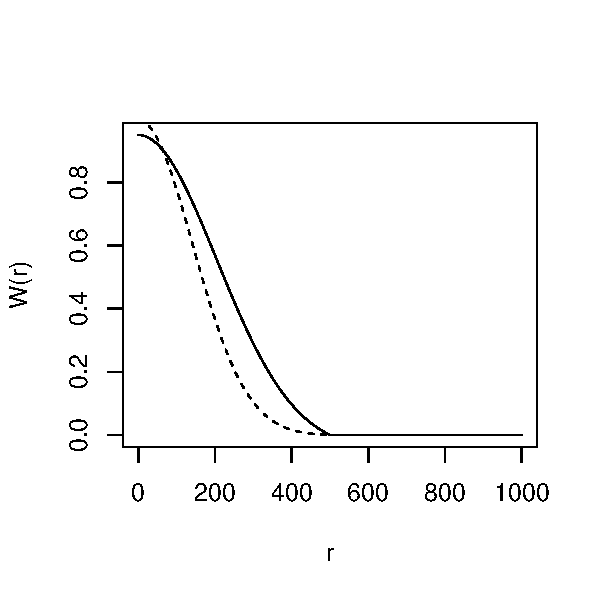
\includegraphics{Meteorology-008}
\end{center}
$R_p$ is automatically adjusted so that it has lower values in data-rich regions and is increased in data-poor regions. The method, however, requires the user to specify $N$, the average number of observations to be included for each target point. $R_p$ is then varied as a smooth function of the local density in such a way that this average is achieved over the spatial domain. Estimation of $R_p$ is as follows:
\begin{enumerate}
\item{A user-specified value is used to initialize $R_p$.}
\item{Interpolation weights $W_i$ are calculated for all $i = (1, ..., n)$ stations, and the local station density is calculated as:
\begin{equation}
D_p = \frac{\sum_{i=1}^{n}{(W_i/\hat{W})}}{\pi \cdot R_p^2}
\end{equation}
where $\hat{W}$ is the average weight over the untruncated region of the kernel, calculated as:
\begin{equation}
\hat{W} = \left( \frac{1 - e^{-\alpha}}{\alpha}\right)- e^{-\alpha}
\end{equation}
}
\item{A new $R_p$ value is calculated as a function of $N$ and $D_p$, as:
\begin{equation}
R_p = \sqrt{\frac{N^*}{D_p \cdot \pi}}
\end{equation}
where $N^* = 2N$ for the first $I - 1$ iterations, and $N^* = N$ for the final iteration.
}
\item{ The new $R_p$ is substituted in step (2) and steps (2-4) are iterated a specified number of times $I$. The final $R_p$ value is used to generate interpolation weights $W_i$.}
\end{enumerate}
Thornton et al. (1997) suggested to use this algorithm only once per point (and variable to be estimated), but since missing meteorological values can occur only in some days, we apply the algorithm for each target point and day. The interpolation method for a given set of observations is defined by four parameters $R$, $I$, $N$ and $\alpha$. Following Thornton et al. (1997), we set $R = 140000$ meters and $I = 3$ by default (see parameters '\texttt{initial\_Rp}' and '\texttt{iterations}' given in function \texttt{defaultInterpolationParams()}). The other parameters ($N$ and $\alpha$) depend on the variable to be interpolated.

\subsection{Temperature}
Predictions for minimum temperature and maximum temperature are done in the same way, so we refer to a general variable $T$. We focus on the prediction of $T_p$, the temperature at a single target point $p$ and for a single day, based on observations $T_i$ and interpolation weights $W_i$ for the $i = (1, ..., n)$ weather stations. Prediction of $T_p$ requires a correction for the effects of elevation differences between observation points $z_1, ..., z_n$ and the prediction point $z_p$. Thornton et al. (1997) established the relationship between elevation and temperature using transformed variables (temporal or spatial moving window averages) for temperature and elevation, instead of the original variables, but we did not implement this feature here. A weighted least-squares regression is used to assess the relationship between temperature and elevation. Instead of regressing $z_i$ on $T_i$, the independent variable is the difference in elevations associated with a pair of stations, and the dependent variable is the corresponding difference in temperatures. This gives a regression of the form:
\begin{equation}
(T_1 - T_2) = \beta_0 + \beta_1 \cdot (z_1 - z_2)
\end{equation}
where subscripts $1$ and $2$ indicate the two stations of a pair and $\beta_0$ and $\beta_1$ are the regression coefficients. Regression is performed using all possible pairs of stations and the regression weight associated with each point is the product of the interpolation weights associated with the stations in a pair. The temperature for the target point, $T_p$ is finally predicted as follows:
\begin{equation}
T_{p} = \frac{\sum_{i=1}^{n}{W_i\cdot (T_i + \beta_0 + \beta_1 \cdot(z_p - z_i))}}{\sum_{i=1}^{n}{W_i}}
\end{equation}
where $z_p$ is the elevation of the target point and $z_i$ is the elevation of the weather station.

\subsection{Relative humidity}
Relative humidity is a parameter not always recorded in weather stations. When input station weather data does not include relative humidity, \texttt{meteoland} estimates it directly from minimum and maximum temperature (Thornton et al. 1997). Assuming that minimum daily air temperature $T_{min,p}$ at the target point is a good surrogate of dew-point temperature $T_{d,p}$ (i.e. $T_{d,p} = T_{min,p}$; note that this assumption may not be valid in arid climates), one can estimate actual vapor pressure $e_{p}$ (in kPa) as:
\begin{equation}
e_{p} = 0.61078 \cdot e^{\left(\frac{17.269\cdot T_{d,p}}{237.3+T_{d,p}}\right)}
\end{equation}
and saturated vapor pressure $e_{s,p}$ (in Pa) as:
\begin{equation}
e_{s,p} = 0.61078 \cdot e^{\left(\frac{17.269\cdot T_{a,p}}{237.3+T_{a,p}}\right)}
\end{equation}
where $T_{a,p} = 0.606 \cdot T_{max,p} + 0.394 \cdot T_{min,p}$ is the average daily temperature. Finally, relative humidity $RH_p$ (in percentage) is calculated as:
\begin{equation}
RH_p = 100 \cdot \frac{e_{p}}{e_{s,p}}
\end{equation}

When relative humidity has been measured at weather stations, interpolation should be preferred to estimation from minimum and maximum temperature. However, because relative humidity depends on temperature, relative humidity $RH_i$ of each weather station $i$ has to be converted to dew-point temperature $T_{d,i}$ before interpolation (Tymstra et al. 2010). To obtain the dew-point temperature one first needs to calculate vapor pressure:
\begin{equation}
e_i = e_{s,i} \cdot (RH_i / 100)
\end{equation}
where $e_{s,i}$ is the saturated water vapor pressure of station $i$, calculated as indicated above. Then, dew-point temperature of station $i$ is obtained from:
\begin{equation}
T_{d,i} = \frac{237.3\cdot \ln(e_i/0.61078)}{17.269 - \ln(e_i/0.61078)}
\end{equation}
Unlike temperature, weighted regression is not used. The dew-point temperature for the target point, $T_{d,p}$ is predicted as:
\begin{equation}
T_{d,p} = \frac{\sum_{i=1}^{n}{W_i\cdot T_{d,i}}}{\sum_{i=1}^{n}{W_i}}
\end{equation}
From the interpolated dew-point temperature one can obtain actual vapour pressure $e_{p}$ and, together with saturated vapour pressure at point $p$, one calculates relative humidity as indicated above. If saturated vapour pressure is referred to average temperature $T_{a,p}$, then relative humidity is average relative humidity $RH_{a,p}$. If, instead, one refers saturated vapour pressure to minimum and maximum daily temperatures one obtains, respectively, maximum and minimum relative humidity values ($RH_{max,p}$, $RH_{min,p}$). After their estimation, the routine checks that the predicted maximum and minimum relative humidity values stay within the physical limits 0\% and 100\%.


\subsection{Precipitation}
Predictions of precipitation are complicated by the need to predict both daily occurrence and, conditioned on this, daily precipitation amount. Thornton et al. (1997) define a binomial predictor of spatial precipitation occurrence as a function of the weighted occurrence at surrounding stations. The precipitation occurrence probability $POP_p$ is:
\begin{equation}
POP_p = \frac{\sum_{i=1}^{n}{W_{o,i}\cdot PO_i}}{\sum_{i=1}^{n}{W_{o,i}}}
\end{equation}
where $PO_i$ is the binomial precipitation occurrence in station $i$ (i.e., $PO_i = 0$ if $P_i = 0$ and $PO_i = 1$ if $P_i > 0$) and $W_{o,i}$ is the interpolation weight for precipitation occurrence. Once $POP_p$ is calculated, then precipitation occurs if $POP_p$ is smaller than a critical value (i.e. $PO_p = 1$ if $POP_p < POP_{crit}$ and $PO_p = 0$ otherwise). 

Conditional on precipitation occurrence we calculate the prediction of daily total precipitation, $P_p$. Like with temperature, Thornton et al. (1997) established the relationship between elevation and precipitation using transformed variables (temporal or spatial moving window averages) for precipitation and elevation. Following their results, we transform precipitation values using a temporal window with side of 5 days. Weighted least-squares, where the weight associated with each point is the product of the interpolation weights associated with the stations in a pair, is used to account for elevation effects on precipitation. Unlike Thornton et al. (1997), who use the same set of interpolation weights (i.e. $W_{o,i}$) for precipitation occurrence and regression, we use a second set of interpolation weights $W_{r,i}$ for the calculation of regression weights. The dependent variable in the regression function is defined as the normalized difference of the precipitation observations $P_i$ for any given pair of stations:
\begin{equation}
\left(\frac{P_1 - P_2}{P_1 + P_2}\right) = \beta_0 + \beta_1 \cdot (z_1 - z_2)
\end{equation}
To obtain the predicted daily total $P_p$ we use the following equation:
\begin{equation}
P_p = \frac{\sum_{i=1}^{n}{W_{o,i}\cdot P_i \cdot PO_i \cdot \left(\frac{1 + f}{1 - f} \right)}}{\sum_{i=1}^{n}{W_{o,i} \cdot PO_i}}
\end{equation}
where $f = \beta_0 + \beta_1 \cdot (z_p - z_i)$. Note the usage of interpolation weight $W_{o,i}$ (and not $W_{r,i}$). The form of prediction requires that $\lvert f \rvert < 1$. A parameter $f_{max}$ (with default $f_{max} = 0.95$ ) is introduced to force $\lvert f \rvert  = f_{max}$ whenever $\lvert f \rvert  > f_{max}$.


\subsection{Wind}
Interpolation of wind characteristics depends on the amount of information available:
\begin{itemize}
\item{Interpolation of wind speed only}
\item{Interpolation of wind vectors (speed and direction)}
\item{Interpolation of wind vectors using wind fields}
\end{itemize}

In the following we detail the calculations in each case.
\subsubsection{Interpolation of wind speed}
The predicted wind speed $u_{p}$ for a target point $p$ is the weighted average of station wind speed values $\{u_{i}\}$  $i=(1,... , n)$ using the interpolation weights $W_i$ determined from the truncated Gaussian filter:
\begin{equation}
u_{p} = \frac{\sum_{i=1}^{n}{W_i \cdot u_{i}}}{\sum_{i=1}^{n}{W_i}}
\end{equation}
\subsubsection{Interpolation of wind vectors}
Interpolation of wind vectors for a target point $p$ is as follows. Let $\mathbf{v}_{i}$ be the wind vector in weather station $i$. $\mathbf{v}_{i}$ is initially expressed using polar coordinates. Indeed, we have $u_{i}$ and $\theta_{i}$, the wind speed and wind direction, respectively. If we express $\mathbf{v}_{i}$ in cartesian coordinates we have:
\begin{equation}
x_{i} = u_{i}\cdot \sin(\theta_{i}) \quad y_{i} = u_{i}\cdot \cos(\theta_{i})
\end{equation}
The predicted wind vector $\mathbf{v}_{p}$ is the weighted average of the wind vectors $\{\mathbf{v}_{i}\}$  $i=(1,... , n)$ predicted for point $p$ using the interpolation weights $W_i$ determined from the truncated Gaussian filter:
\begin{equation}
x_{p} = \frac{\sum_{i=1}^{n}{W_i \cdot x_{i}}}{\sum_{i=1}^{n}{W_i}}  \quad y_{p} = \frac{\sum_{i=1}^{n}{W_i \cdot y_{i}}}{\sum_{i=1}^{n}{W_i}}
\end{equation}
The polar coordinates of the predicted wind vector $\mathbf{v}_{p}$  are:
\begin{equation}
u_{p} = \sqrt{x^{2}_{p} + y^{2}_{p}} \quad \theta_{p} = \tan^{-1}(x_{p}/y_{p})
\end{equation}

\subsubsection{Interpolation of wind vectors using wind fields}
More precise wind interpolation of wind vectors requires a set of static wind fields covering the landscape of interest. Each of these wind fields has been calculated assuming a domain-level combination of wind speed and wind direction. The set of domain-level combinations should cover all possible winds in the landscape under study. For example, one could decide to include the combinations of eight different wind directions (i.e., N, NE, E, SE, ...) and three wind speed classes. The wind estimation of a given target point depends on both the wind observations at weather stations and these static wind fields.

In a given day (and before processing target points) we begin by identifying, for each weather station $i = (1, ... ,n)$, the wind field $m_i$ corresponding to a minimum difference between the observed wind vector $\mathbf{v}_i$ and the wind vector of the station in the wind field (i.e., minimum distance between the corresponding cartesian coordinates). The set of wind fields $\{m_i\}$ $i = (1, ... ,n)$ chosen for each weather station conform the information for wind interpolation in a given day.

Actual wind interpolation details for a target point $p$ are as follows. We first draw for each $i=(1,... , n)$ the wind vector $\mathbf{v}_{m_i,p}$ corresponding to the location of the target point $p$ in wind fields $m_i$. Let $u_{m_i,p}$ and $\theta_{m_i,p}$ be the wind speed and wind direction of $\mathbf{v}_{m_i,p}$, respectively. The cartesian coordinates of $\mathbf{v}_{m_i,p}$ are:
\begin{equation}
x_{m_i,p} = u_{m_i,p}\cdot \sin(\theta_{m_i,p}) \quad y_{m_i,p} = u_{m_i,p}\cdot \cos(\theta_{m_i,p})
\end{equation}
The predicted wind vector $\mathbf{v}_{p}$ is the weighted average of the wind vectors $\{\mathbf{v}_{m_i,p}\}$  $i=(1,... , n)$ predicted for point $p$ using the interpolation weights $W_i$ determined from the truncated Gaussian filter:
\begin{equation}
x_{p} = \frac{\sum_{i=1}^{n}{W_i \cdot x_{m_i,p}}}{\sum_{i=1}^{n}{W_i}}  \quad y_{p} = \frac{\sum_{i=1}^{n}{W_i \cdot y_{m_i,p}}}{\sum_{i=1}^{n}{W_i}}
\end{equation}
The polar coordinates of the predicted wind vector $\mathbf{v}_{p}$  are found as before.


\section{Estimation of solar radiation}
Incident daily solar radiation is not interpolated, but estimated from topography and measurements of temperature, humidity and precipitation.


\subsection{Solar declination and solar constant}
The declination of the sun $\delta$ is the angle between the rays of the sun and the plan of the Earth's equator. Solar declination varies with years and seasons. However, the Earth's axial tilt changes slowly over thousands of years but it is nearly constant for shorter periods, so the change in solar declination during one year is nearly the same as during the next year. Solar constant ($I_0$) is normally given a nominal value of 1.361 kW·m$^{-2}$ but in fact it also varies through the year and over years. Both can be calculated from Julian day ($J$), the number of days number of days since January 1, 4713 BCE at noon UTC. from Julian day. In \texttt{meteoland}, julian days, solar declination and solar constant are calculated using an adaptation of the code as in package \texttt{insol} (by J.G. Corripio), which is based on Danby (1988) and Reda \& Andreas (2003). 

The following figures show the variation of solar declination and the value of solar constant over a year (see functions \texttt{radiation\_solarDeclination()} and \texttt{radiation\_solarConstant()}):

\begin{center}
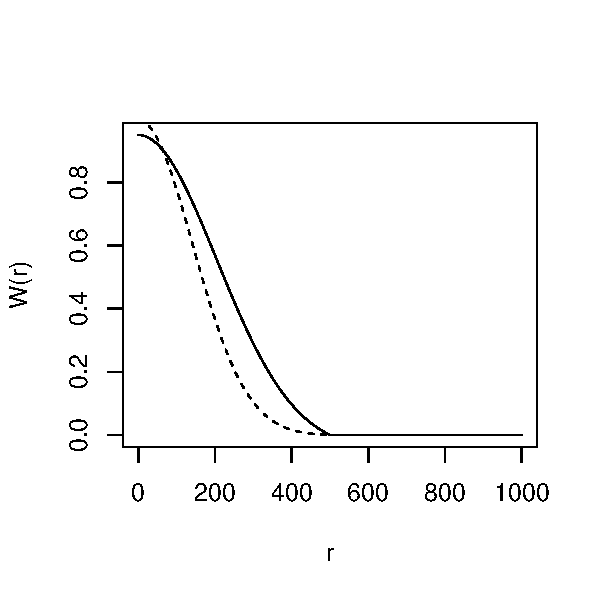
\includegraphics{Meteorology-010}
\end{center}

\subsection{Day length}
Calculation of sunrise and sunset on a horizontal surface is rather straightforward. The hour angles of sunrise and sunset ($sr$ and $ss$, both in radians) for a horizontal surface of latitude $\phi$ on a day with declination $\delta$ (both expressed in radians) are:
\begin{eqnarray}
sr &=& T_1 = \cos^{-1}\left(\max(\min(-\tan(\phi) \cdot \tan(\delta),1),-1)\right) \\
ss &=& T_0 = - T_1
\end{eqnarray}
Knowing that each hour corresponds to 15 degrees of rotation, hour angles can be transformed to solar hours. The following figures show the seasonal variation of sunrise and sunset hours, as well as day length, for horizontal surfaces in three latitudes (40North, equator and 40South) (see functions \texttt{radiation\_sunRiseSet()} and  \texttt{radiation\_daylength()}):
\begin{center}
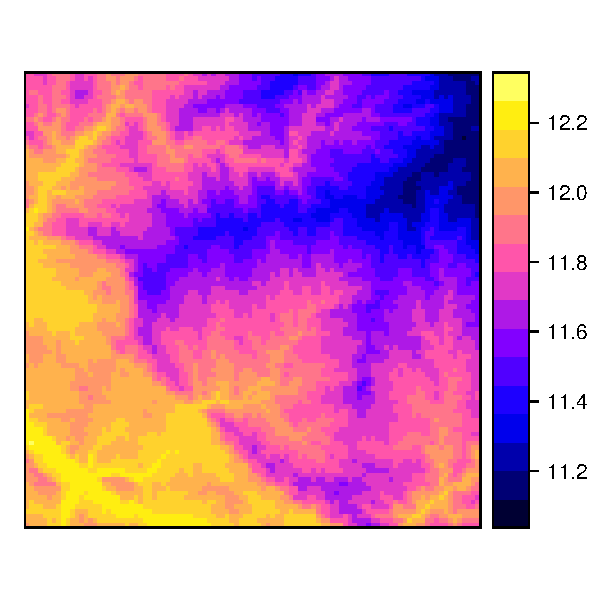
\includegraphics{Meteorology-011}
\end{center}

For inclinated slopes, the calculation of day length is based on the concept of equivalent slopes, which are places on earth where the slope of earth's surface is equal to the slope of interest. The calculations start with the determination of the latitude $L_1$ of the equivalent slope:
\begin{eqnarray}
  L_1 &=& \sin^{-1}\left(\cos(Z_x)\cdot \sin(\phi)+\sin(Z_x) \cdot \cos(\phi) \cdot \cos(A)\right) \\
  D &=& \cos(Z_x) \cdot \cos(\phi)-\sin(Z_x) \cdot \sin(\phi) \cdot \cos(A)
\end{eqnarray}
where $\phi$ is the latitude, $A$ is the azimuth of the slope (aspect) and $Z_x$ is the zenith angle of the vector normal to the slope (equal to the slope angle). Then $L_2$ is defined depending on the value of $D$. If $D < 0$ then:
\begin{equation}
  L_2 = \tan^{-1}\left(\frac{\sin(Z_x) \cdot \sin(A)}{D}\right)+\pi
\end{equation}
Otherwise, $L_2$ is calculated as:
\begin{equation}
L_2 =  \tan^{-1}\left(\frac{\sin(Z_x) \cdot \sin(A)}{D}\right)
\end{equation}
Once $L_1$ and $L_2$ are available, we can calculate solar hours on equivalent slopes:
\begin{eqnarray}
  T_7 &=& \cos^{-1}\left(\max(\min(-\tan(L_1) \cdot \tan(\delta), 1),-1)\right)-L2 \\ 
  T_6 &=& - \cos^{-1}\left(\max(\min(-\tan(L_1) \cdot \tan(\delta), 1),-1)\right) -L2 
\end{eqnarray}
Being $T_6$ and $T_7$ the hour angle of sunrise and sunset on equivalent slopes, respectively. 
and the hour angles of sunrise ($sr$) and sunset ($ss$) on the slope (both in radians) are found comparing the hour angles on equivalent surfaces with the hour angles on the horizontal surface:
\begin{eqnarray}
  sr &=& \max(T_0,T_6) \\
  ss &=& \min(T_1,T_7)
\end{eqnarray}

The following three figures show the seasonal variation of sunrise and sunset hours, as well as day length, for slopes of 30 inclination, facing to the four cardinal points. Curves for flat surfaces are shown for comparison. If the slopes are at latitude 40North:
\begin{center}
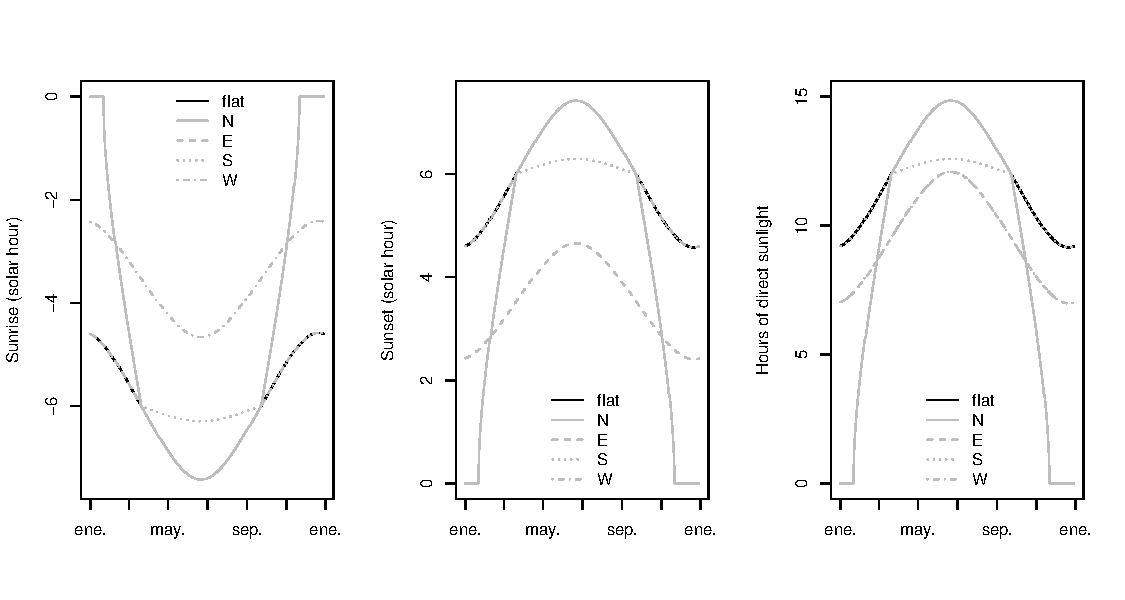
\includegraphics{Meteorology-012}
\end{center}
whereas if they are at Equator (i.e. $\phi = 0$):
\begin{center}
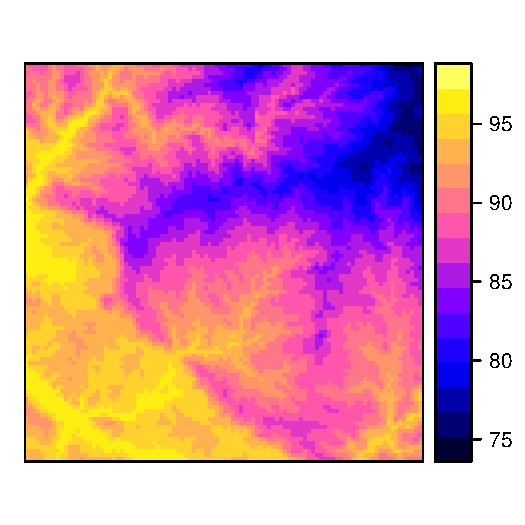
\includegraphics{Meteorology-013}
\end{center}
and if they are at latitude 40South:
\begin{center}
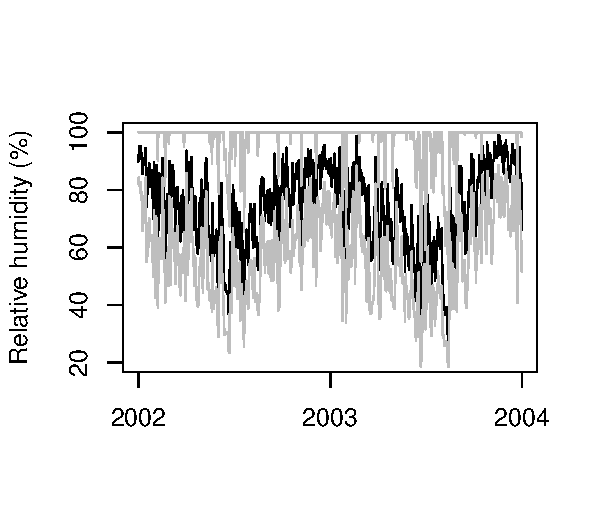
\includegraphics{Meteorology-014}
\end{center}

\subsection{Potential radiation}
Potential solar radiation is the radiation that a surface on earth would receive if atmosphere was not present (i.e. without the effects of cloud reflection, scattering, ...). In \texttt{meteoland}, potential solar radiation is estimated from solar declination, latitude, aspect and slope according to Granier \& Ohmura (1968). Daily potential radiation ($R_{pot}$, in MJ·m$^{-2}$) is calculated by integrating instantaneous potential radiation $R_{pot,s}$ (in kW·m$^{-2}$) over the day between sunrise ($sr$) and sunset ($ss$), using 10 min (i.e. 600 sec) intervals:
\begin{equation}
R_{pot} = \frac{1}{1000}\cdot \sum_{s = sr}^{ss}{600 \cdot R_{pot,s}}
\end{equation}
In turn, instantaneous potential solar radiation $R_{pot,s}$ is calculated using:
\begin{eqnarray}
R_{pot,s} &=& I_0 \cdot [(\sin{\phi}\cdot \cos{H})(-\cos{A}\cdot \sin{Z_x})  -\sin{H}\cdot (\sin{A}\cdot \sin{Z_x}) \nonumber \\
 & & + [(\cos{\phi}\cdot \cos{H})\cdot \cos{Z_x}]\cdot \cos{\delta} \nonumber \\
 & & + [\cos{\phi}\cdot (\cos{A}\cdot \sin{Z_x})+ \sin{\phi}\cdot \cos{Z_x}]\cdot \sin{\delta}]
\end{eqnarray}
where $I_0$ is the solar constant, $\phi$ is the latitude, $H$ is the hour angle measured from solar noon, positively towards the west, $A$ is the azimuth of the slope (aspect), $Z_x$ is the zenith angle of the vector normal to the slope (equal to the slope angle) and $\delta$ is the sun's declination. Note that in the case of a flat surface the previous equation reduces to:
\begin{equation}
R_{pot,s} = I_0 \cdot [\cos{\phi}\cdot \cos{H}\cdot \cos{\delta} + \sin{\phi}\cdot \sin{\delta}]= I_0 \cdot \sin{\beta}
\end{equation}
where $\beta$ is called the solar elevation angle.

The following figures illustrate seasonal variation of potential solar radiation for the horizontal inclinated surfaces presented above (see function \texttt{radiation\_potentialRadiation()}):

\begin{center}
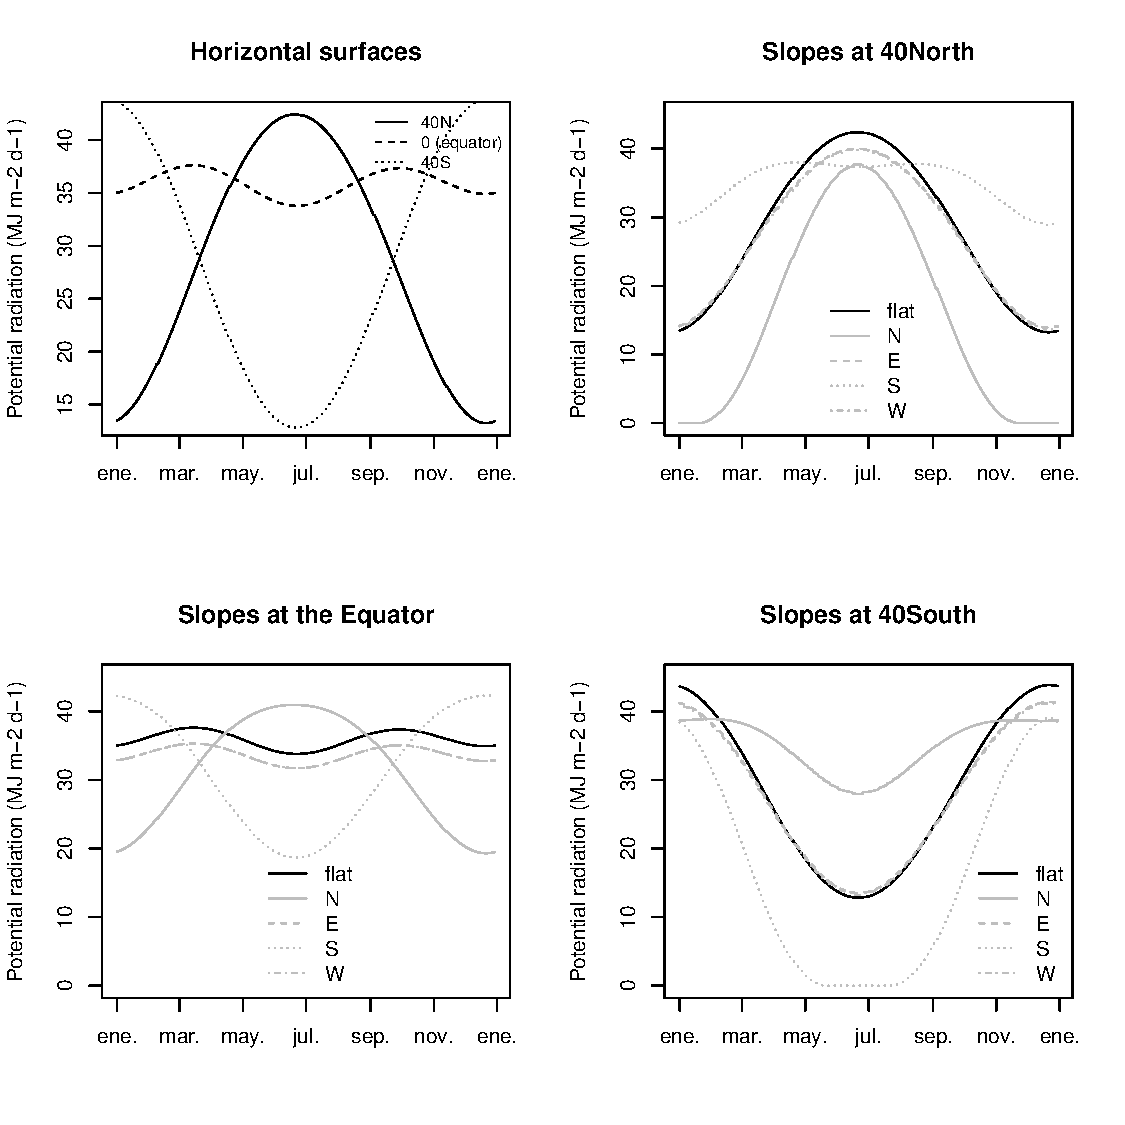
\includegraphics{Meteorology-015}
\end{center}


\subsection{Incident solar radiation}
Incident solar radiation is the amount of (direct) solar radiation reaching the surface after accounting for the atmosphere. Improving the method proposed in Thornton et al. (1997), Thornton \& Running (1999) calculate incident daily total solar radiation $R_{g}$ as:
\begin{equation}
R_g = R_{pot} \cdot T_{t,max} \cdot T_{f,max}
\end{equation}
where $T_{t,max}$ is the maximum (cloud-free) daily total transmittance and $T_{f,max}$ is the proportion of $T_{t,max}$ realized on a given day (cloud correction). The maximum daily total transmittance $T_{t,max}$ is estimated as:
\begin{equation}
T_{t,max} = \left[\frac{\sum_{s = sr}^{ss}{R_{pot,s} \cdot \tau^{(P_z/P_0)\cdot m_{\theta}}}}{\sum_{s = sr}^{ss}{R_{pot,s}}}\right] + (\alpha_{e_p} \cdot {e_p})
\end{equation}
where $\tau = 0.87$ is the instantaneous transmittance at sea level, at nadir, for a dry atmosphere; ${e_p}$ is the actual water vapor pressure (in kPa), estimated as explained before; $\alpha_{e_p} = -6.1\cdot 10^{-2}$kPa$^{-1}$ is a parameter describing the effect of vapour pressure on $T_{t,max}$; $m_{\theta} = 1/\cos{\theta}$ is the optical air mass at solar zenith angle $\cos(\theta) = \sin{\phi}\cdot \sin{\delta}+\cos{\phi}\cdot \cos{\delta} \cdot \cos{H}$; and $P_z/P_0$ is the ratio between air pressure at elevation $z_p$ and air pressure at the sea level, calculated as:
\begin{equation}
(P_z/P_0) = (1.0 -2.2569\cdot 10^{-5}\cdot z_p)^{5.2553}
\end{equation}
In turn, $T_{f,max}$ was empirically related to $\Delta T = T_{\max} - T_{\min}$, the difference between maximum and minimum temperatures for the target point:
\begin{equation}
T_{f,max} = 1.0 - 0.9\cdot e^{-B \cdot {\Delta T}^{C}}
\end{equation}
being $C = 1.5$ and $B$ calculated from:
\begin{equation}
B = b_0 + b_1 \cdot e^{-b_2 \cdot {\hat{\Delta T}}}
\end{equation}
with $b_0 = 0.031$, $b_1 = 0.201$ and $b_2 = 0.185$. In this last equation,  $\hat{\Delta T}$ is a 30-day moving average for the temperature range $\Delta T$. For computational reasons, we do not estimate $\hat{\Delta T}$ from the 30-day moving window average of predicted $\Delta T$ values, but from the interpolation of pre-calculated $\hat{\Delta T}$ values in weather stations. On wet days (i.e. if $P_p > 0$) the estimation of $T_{f,max}$ is multiplied by a factor of $0.75$ to account for clouds.

Although the calculation of incident solar radiation can be done independently of interpolation (see function \texttt{radiation\_solarRadiation()}), it is automatically done in functions \texttt{interpolationpoints()} and \texttt{interpolationgrid()}. 

\subsection{Outgoing longwave radiation and net radiation}
Potential and actual evapotranspiration calculations require estimating the energy actually absorved by evaporating surfaces. Daily net radiation $R_n$ (in $MJ\cdot m^{-2}\cdot day^{-1}$) is calculated using:
\begin{equation}
R_n = R_s\cdot (1 - \alpha) - R_{nl}
\end{equation}
where $R_s$ is the input solar radiation (in $MJ\cdot m^{-2}\cdot day^{-1}$), $\alpha = 0.08$ accounts for surface albedo, and $R_{nl}$ is the net longwave radiation. Outgoing longwave radiation is the radiation emitted by earth. Following McMahon et al. (2013) to obtain $R_{nl}$ one first calculates clear sky radiation $R_{so}$ using:
\begin{equation}
  R_{so} = (0.75 + \cdot 0.00002 \cdot z) \cdot R_{pot}
\end{equation}
where $z$ is elevation and $R_{pot}$ is potential radiation. $R_{nl}$ is then calculated using:
\begin{equation}
R_{nl} = \sigma \cdot (0.34 - 0.14 \cdot \sqrt{e}) \cdot \frac{T_{\max}^4 + T_{\min}^4}{2} \cdot (1.35 \cdot \min(\frac{R_s}{R_{so}},1.0) - 0.35)
\end{equation}
where $e$ is the actual vapor pressure (kPa), $T_{\max}$ and $T_{\min}$ are the maximum and minimum temperatures (in Kelvin) and $\sigma = 4.903\cdot 10^{-9}$ MJ·K$^{-4}$·m$^{-2}$ is the Stephan-Boltzmann constant.

The following figure shows an example of radiation balance for a whole year for a single site (see functions \texttt{radiation\_outgoingLongwaveRadiation()} and \texttt{radiation\_netRadiation()}):
\begin{center}
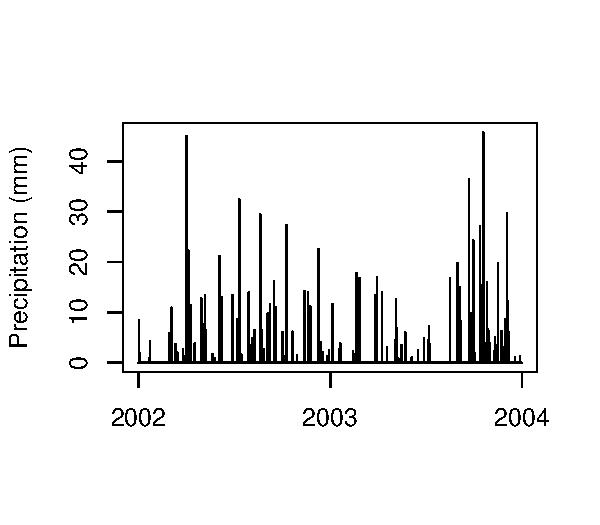
\includegraphics{Meteorology-016}
\end{center}

\subsection{Diurnal trends in diffuse and direct radiation}
Ecological studies sometimes require radiation information at a subdaily scale. This is particularly true for modeling studies that need to calculate canopy photosynthesis. Although meteoland has been designed to assist studies requiring meteorological data at daily scale, a function called \texttt{radiation\_directDiffuseDay()} is provided to divide daily radiation into instantaneous direct and diffuse radiation. Values of instantaneous direct and diffuse radiation (shortwave and photosynthetic active radiation) are calculated following Spitters et al. (1986). First, the ratio between daily diffuse and global radiation ($R_{d}/R_{g}$) is inferred from the ratio between daily potential and global radiation ($R_{g}/R_{pot}$):
\begin{eqnarray}
R_{d}/R_{g} = 1 & & R_{g}/R_{pot}<0.07\\
R_{d}/R_{g} = 1-2.3\cdot (R_{g}/R_{pot}-0.7)^2 & & 0.07\leq R_{g}/R_{pot} <0.35\\
R_{d}/R_{g} = 1.33-1.46\cdot R_{g}/R_{pot} & & 0.35\leq R_{g}/R_{pot} <0.75\\
R_{d}/R_{g} = 0.23 & & 0.75\leq R_{g}/R_{pot}
\end{eqnarray}
In a clear day (e.g. not rainy) the ratio is modified to account for the circumsolar part of diffuse radiation:
\begin{equation}
R'_{d}/R_{g} = \frac{R_{d}/R_{g}}{1+(1- (R_{d}/R_{g})^2)\cdot \cos^2(\pi/4-\beta)\cdot \cos^3\beta} 
\end{equation}
where $\beta$ is the solar elevation angle. Otherwise $R'_{d}/R_{g} = R_{d}/R_{g}$. The daily diffuse shortwave radiation ($R_{d}$) is found by multiplying global radiation by the (modified) ratio:
\begin{equation}
R_{d} = R_{g} \cdot (R'_{d}/R_{g}) 
\end{equation}
The diurnal trend of the irradiance is derived from the daily global radiation and the daily course of potential (i.e. extra-terrestrial) radiation. If we assume that the atmospheric transmission is constant during the daylight period:
\begin{equation}
R_{g,s}/R_{pot,s} =R_{g}/R_{pot}
\end{equation}
this leads to an estimation of the instantaneous global radiation (assuming compatible units):
\begin{equation}
R_{g,s} = R_{g}\cdot (R_{pot,s}/R_{pot})
\end{equation}
and the instantaneous diffuse and direct beam fluxes are estimated using:
\begin{eqnarray}
R_{d,s} &=& R_{d}\cdot (R_{pot,s}/R_{pot}) \\
R_{b,s} &=& R_{g,s} - R_{d,s}
\end{eqnarray}
The whole procedure to calculate direct and diffuse radiation depends on the solar elevation angle, which changes through the day. Although $R'_{d}/R_{g}$ is formulated as a ratio of daily values, the ratio needs to be calculated for every instant, as $R_{pot,s}$.

The procedure for photosynthetic active radiation (PAR) is similar. Daily PAR is assumed to be half of daily global radiation (i.e. $R_{PAR} = 0.5 \cdot R_{g}$. The scattered diffuse component of PAR is bigger than that of global radiation, and the ratio of diffuse over total PAR radiation is:
\begin{equation}
R_{PAR,d}/R_{PAR} = \left[1+0.3 \cdot (1- (R_{d}/R_{g})^2)\right]\cdot  (R'_{d}/R_{g})
\end{equation}
The ratio $R_{PAR,d}/R_{PAR}$ is used to determine daily diffuse PAR and the calculation of instant rates are the same as for global radiation.

To illustrate the above calculations, we assume a target location in a flat terrain located at 42N latitude and 100 m.a.s.l, having 30 MJ·m$^{-2}$ of daily global radiation on the 2001/June/01, the hourly variation in diffuse and direct radiation would be:
\begin{center}
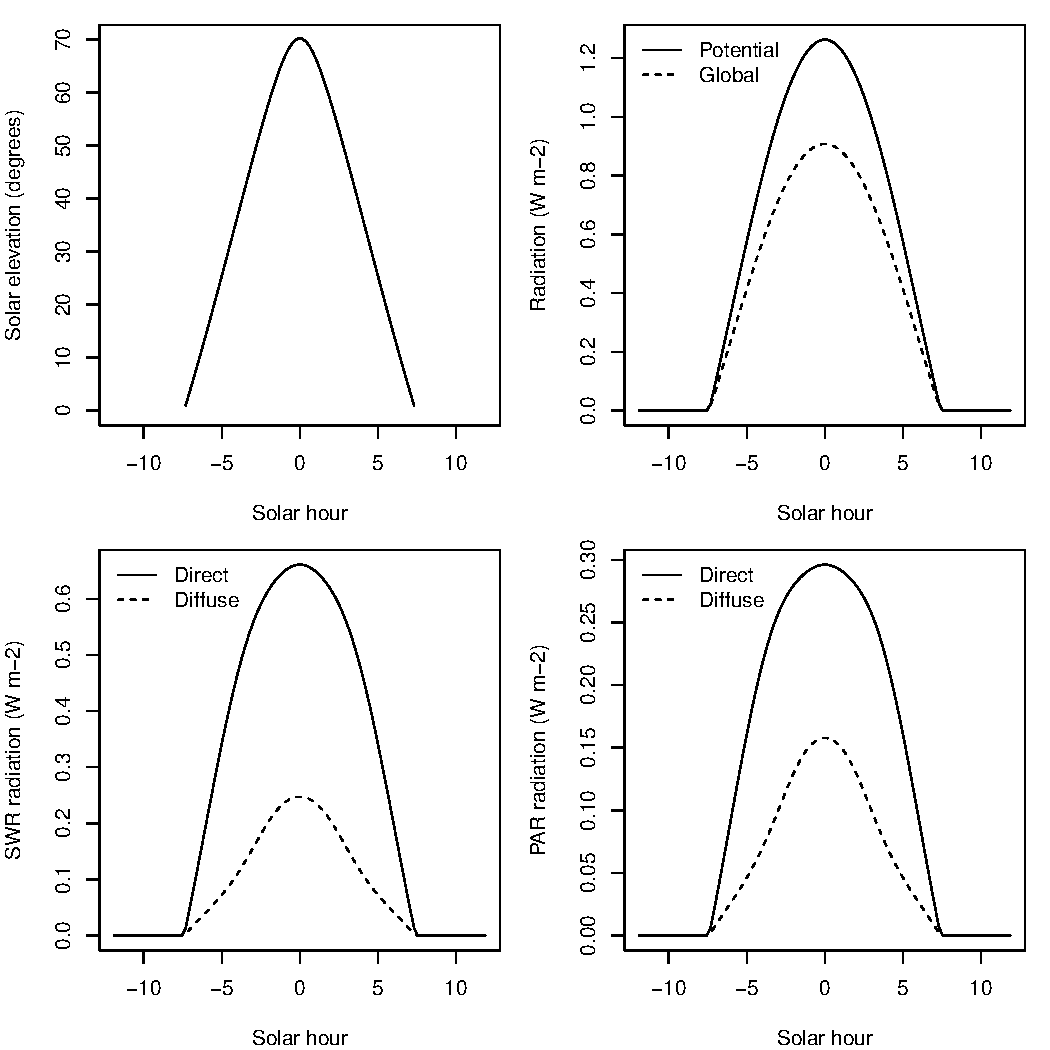
\includegraphics{Meteorology-017}
\end{center}
\section{Statistical correction of weather data}
Statistical correction is necessary when meteorological data is available at a spatial scale that is too coarse for landscape-level analysis. This is usually the case when taking predictions from global or regional climate models. The general idea of correction to the landscape level is that a fine-scale meteorological series is to be compared to coarse-scale series for the a historical (reference) period. The result of this comparison can be used to correct coarse-scale meteorological series for other periods (normally future projections). In the case of most meteorological variables, the comparison consists in calculating a bias using the reference period and applying this bias to the future period. However, in the case of precipitation a different procedure is needed.

\subsection{Precipitation}
There are several approaches to correct precipitation predictions of climate models. Among the most popular approaches are statistical transformations that that aim to adjust aspects of the distribution of predicted values so that the new distribution resembles observations. A common approach is to use cumulative distribution function (CDF) of observed and modelled values. In \texttt{meteoland} we perform quantile mapping by calling the functions implemented in package \texttt{qmap} (Gudmundsson et al. 2012). In short, the empirical CDFs are approximated using tables of empirical percentiles. Values in between the percentiles are approximated using linear interpolation. If new model values (e.g. from climate projections) are larger than the training values used to estimate the empirical CDF, the correction found for the highest quantile of the training period is used. 

Quantile mapping is done month by month, to account for seasonal variation of precipitation distribution in the target area. The following figures show the correction of RCM precipitation predictions for 2023 using interpolated data from 2002-2003 as observations for the reference period. Note that at least 15 years of observations (and not two!) would be needed for a correct estimation of monthly CDFs.
\begin{center}
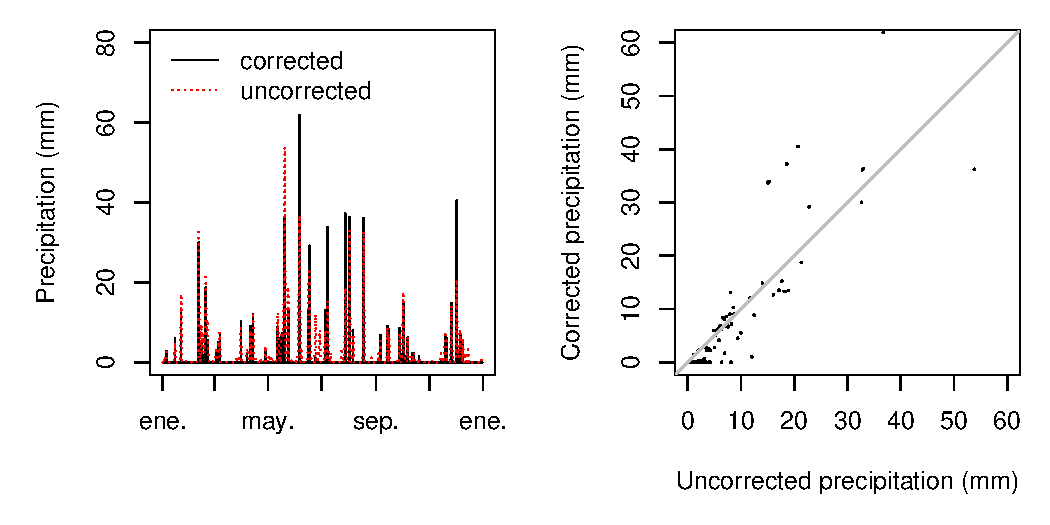
\includegraphics{Meteorology-019}
\end{center}
\subsection{Temperature}
Let $x$ be the meteorological variable observed for the target point in the reference period, and $u$ the same variable, but estimated at the coarse-scale for the reference period. Month $m$ bias of the coarse-scale data ($\theta_{m}$) is the average of the difference between $u$ and $x$ over all $n_m$ days of month $m$ in the reference period:
\begin{equation}
\theta_{m} = \sum_{i=1}^{n_m}{(u_i-x_i)}/n_m
\end{equation}
Month biases are used to correct the coarse-scale value of day $i$ in the projected period using:
\begin{equation}
c_i = u_i - \theta_{m(i)}
\end{equation}
where $m(i)$ is the month of day $i$.

Mean daily temperature is corrected by the simple bias correction explained above (i.e. $x = T_{mean, obs}$ and $u = T_{mean, est}$):
\begin{equation}
T_{mean, cor} = T_{mean, est} - \theta_{m(i)}
\end{equation}
To correct minimum (respectively maximum) temperature values, the unbiasing method described for mean temperature could lead to estimates being above (resp. below) the daily average. To avoid this source of potential inconsistency, a multiplicative scaling factor (found by regression through the origin) is instead applied to the difference between minimum (resp. maximum) temperature and mean temperature. First, we define $x$ and $u$ as the difference in temperature ($\delta$):
\begin{eqnarray}
x &=& \delta_{min, obs} = T_{min, obs} - T_{mean, obs}\\
u &=& \delta_{min, est} = T_{min, est} - T_{mean, est}
\end{eqnarray}
Then, for each month $m$ we regress $x$ on $u$ forcing a zero intercept. This gives a multiplicative (i.e. scaling) factor $\eta_{m}$ that we can use to perform the correction:
\begin{equation}
T_{min, cor} = T_{mean, cor} + \delta_{min, est} \cdot \eta_{m(i)}
\end{equation}

The following figures show the correction of RCM mean, minimum and maximum temperature predictions for 2023 using interpolated data from 2002-2003 as observations for the reference period:
\begin{center}
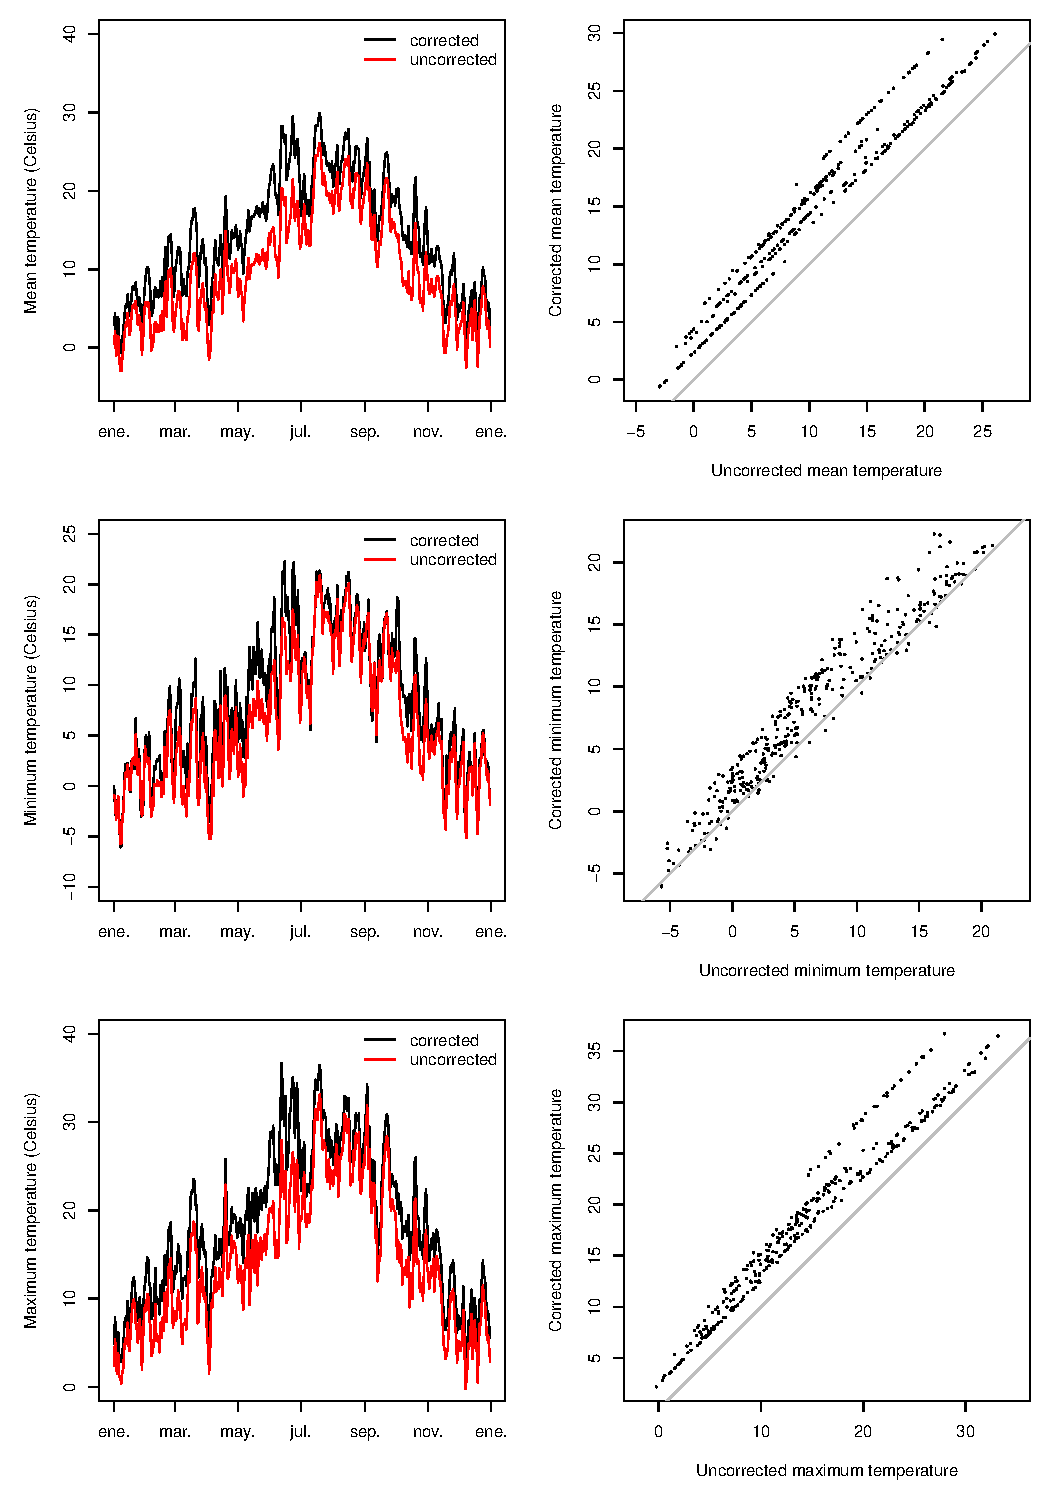
\includegraphics{Meteorology-020}
\end{center}

\subsection{Other variables}
Radiation and wind speed are corrected using the unbiasing procedure described for mean temperature. In the case of relative humidity, values are transformed to specific humidity, bias correction is applied to this variable and the result is back-transformed to relative humidity. Since historic wind data is often not available, if wind speed data is missing the coarse-scale wind estimate is taken directly without correction.

The following figures show the correction of RCM radiation predictions for 2023 using interpolated data from 2002-2003 as observations for the reference period:
\begin{center}
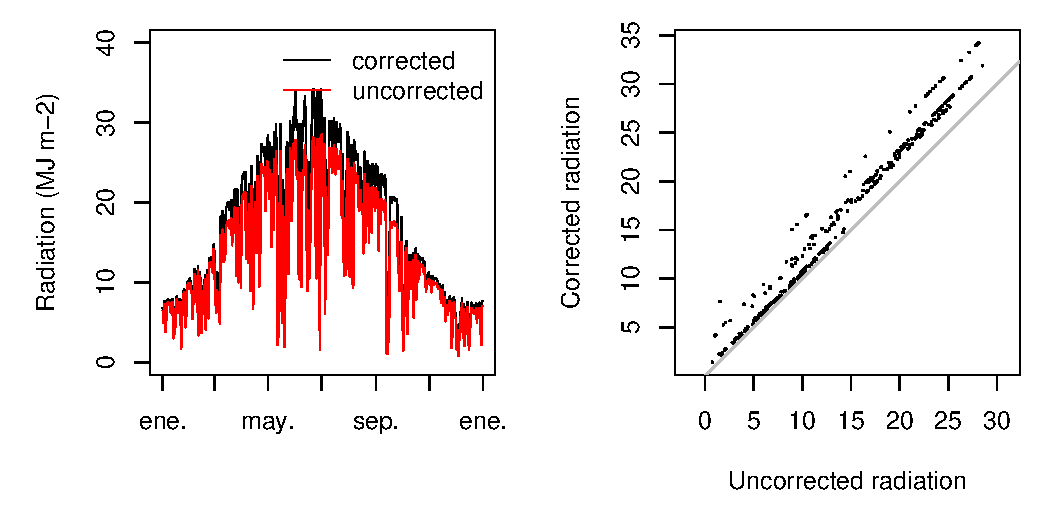
\includegraphics{Meteorology-021}
\end{center}



\section{Estimation of potential evapo-transpiration}
Package \texttt{meteoland} allows calculating daily potential evapo-transpiration (PET) using Penman's formulation (Penman 1948; 1956) or Penman-Monteith formulation. PET is automatically calculated after meteorological data have been interpolated (i.e. within functions \texttt{interpolationpoints()} and \texttt{interpolationgrid()}) or downscaled (i.e. within functions \texttt{correctionpoints()} and \texttt{correctiongrid()}), but PET values can also be calculated for a single point using functions \texttt{penman()} or \texttt{penmanmonteith()}. For other formulations of PET, the reader is referred to package \texttt{`Evapotranspiration'}.

\subsection{Penman formulation}
Penman (1948) proposed an equation to calculate daily potential evaporation that combined an energy equation based on net incoming radiation with an aerodynamic approach. The Penman or Penman combination equation is:
\begin{equation}
E_{pot} = \frac{\Delta}{\Delta+\gamma}\cdot \frac{R_n}{\lambda}+\frac{\lambda}{\Delta + \lambda}\cdot E_a
\end{equation}
where $PET$ is the daily potential evaporation (in $mm \cdot day^{-1}$) from a saturated surface, $R_{n}$ is the daily radiation to the evaporating surface (in $MJ\cdot m^{-2}\cdot day^{-1}$), $\Delta$ is the slope of the vapour pressure curve ($kPa\cdot \degree C^{-1}$) at air temperature, $\gamma$ is the psychrometric constant ($kPa\cdot \degree C^{-1}$), and $\lambda$ is the latent heat of vaporization (in $MJ\cdot kg^{-1}$). $E_a$  (in $mm \cdot day^{-1}$) is a function of the average daily windspeed ($u$, in $m\cdot s^{-1}$), and vapour pressure deficit ($D$, in $kPa$):
\begin{equation}
E_a = f(u) \cdot D = f(u) \cdot (v_a^*-v_a)
\end{equation}
where $v_a^*$ is the saturation vapour pressure ($kPa$) and $v_a$ the actual vapour pressure ($kPa$) and $f(u)$ is a function of wind speed, for which there are two alternatives (Penman 1948; 1956):
\begin{eqnarray}
f(u) &=& 1.313 + 1.381 \cdot u\\
f(u) &=& 2.626 + 1.381 \cdot u
\end{eqnarray}
If wind speed is not available, an alternative formulation for $E_{pot}$ is used as an approximation (Valiantzas 2006):
\begin{equation}
PET \simeq 0.047\cdot R_s \cdot (T_a+9.5)^{0.5}-2.4\cdot (\frac{R_s}{R_{pot}})^2+0.09\cdot(T_a-20)\cdot(1-\frac{RH_{mean}}{100})
\end{equation}
where $R_s$ is the incoming solar radiation (in $MJ\cdot m^{-2}\cdot day^{-1}$), $T_a$ is the mean daily temperature (in $\degree C$), $R_{pot}$ is the potential (i.e. extraterrestrial) solar radiation (in $MJ\cdot m^{-2}\cdot day^{-1}$) and $RH_{mean}$ is the mean relative humidity (in percent). 


\subsection{Penman-Monteith formulation}
The Penman-Monteith combination equation:
\begin{equation}
E_{pot} = \frac{1}{\lambda} \cdot \frac{\Delta \cdot R_{n} + D \cdot (\rho \cdot C_p/r_a)}{\Delta + \gamma \cdot (1 + r_c/r_a)}
\end{equation}
where  $D$ is the vapour pressure deficit (in kPa), $\Delta$  is the slope of the saturated vapor pressure (in $Pa \cdot K^{-1}$), $\gamma$ is the psychrometer constant (in $kPa\cdot K^{-1}$), $\lambda$ is the latent heat vaporization of water (in $MJ\cdot kg^{-1}$) and $C_p$ is the specific heat of air (in $MJ\cdot kg^{-1}\cdot K^{-1}$). $r_c$ is the canopy resistance (in $s\cdot m^{-1}$). For simplicity, aerodynamic resistance ($r_a$) is currently set to $r_a = 208.0/u$ where $u$ is the input wind speed.  

\section{Miscellaneous functions}
\subsection{Downloading data from AEMET}

National meteorological agencies are increasingly adopting an open data philosophy and one of them is the Spanish meteorological agency (Agencia Española de Meteorología, AEMET). In \texttt{meteoland} we provide two functions that retrieve AEMET data using their OpenData API (API keys need to be obtained from AEMET):
\begin{itemize}
\item{\texttt{downloadAEMETstationlist()} : Gets the list of stations from which daily meteorological data is available.}
\item{\texttt{downloadAEMETpoints()} : Downloads historical daily meteorological data corresponding to a input set of stations and period.}
\item{\texttt{downloadAEMETcurrentday()} : Downloads and averages last 24h of meteorological data corresponding to a input set of stations.}
\end{itemize}


\subsection{Extraction of climatic netCDF data}

\textbf{NetCDF} is a standard data format for meteorological data. In particular, this format is used to store the predictions of global and regional climate models. Function \texttt{extractNetCDF()} parses a set of \textbf{NetCDFs} and extracts the daily meteorological data of a landscape boundary box for use within \texttt{meteoland}. The function first identifies which cells in NetCDF data should be extracted (according to the input boundary box), and the overall period. For each cell to be processed, the function loops over all files (which can describe different variables and time periods) and extracts the corresponding data. The function transforms units to the units used in meteoland. If specific humidity and mean temperature are available, the function also calculates mean relative humidity.

\subsection{Obtaining static wind fields}
External software is necessary to calculate the set of wind fields for the study area under different domain-level average situations. For this we recommend using \textbf{\href{http://firelab.org/project/windninja}{WindNinja}}, a computer program that calculates spatially varying wind fields for wildland fire applications. WindNinja allows simulating the spatial variation of wind for one instant in time. It was developed to be used by emergency responders within their typical operational constraints of fast simulation times (seconds), low CPU requirements (single processor laptops), and low technical expertise. WindNinja is typically run on domain sizes up to 50 kilometers by 50 kilometers and at resolutions of around 100 meters. The program is free and can be downloaded from \href{http://www.firemodels.org}{www.firemodels.org}.

The inputs for a basic run of WindNinja are an elevation data file for the study area, a domain-averaged input wind speed and direction and a specification of the dominant vegetation in the area. In order to obtain a set of pre-computed rasters of wind direction and speed, we suggest the following procedure:
\begin{itemize}
\item{Export the elevation raster of the study area in one of the file formats accepted by WindNinja (`.asc', `.tif' or `.img'). In the case of a large study area (e.g. > 100 x 100 km) one should run WindNinja in subsets of the area and then integrate the results (e.g., Sanjuan et al. 2014).}
\item{Run WindNinja, using the elevation of the study area, for all combinations of wind direction and wind speed class (for each wind speed class an mean class value has to be chosen). Several combinations of domain-level wind speed and wind direction can be specified for a single run, and the program can also be run in batch mode.}
\item{Read raster files created by WindNinja (a wind speed file, a wind direction file) for each combination of domain-level wind speed and direction. }
\end{itemize}
Function \texttt{readWindNinjaOutput()} can be used to conduct this last step. The function allows parsing all the ASCII raster files produced by WindNinja for combinations of wind direction (e.g., 0, 45, 90, 135, 180, 225, 270 and 315 degrees) and wind speed (e.g., 2, 7 and 10 m/s). The function returns a list with the following elements:
\begin{itemize}
\item{The vector of domain-level wind directions corresponding to WindNinja Runs}
\item{The vector of domain-level wind speed corresponding to WindNinja Runs}
\item{An object \texttt{SpatialGridDataFrame} containing the wind directions (in degrees from North) for all WindNinja runs.}
\item{An object \texttt{SpatialGridDataFrame} containing the wind speeds (in m/s) for all WindNinja runs.}
\end{itemize}


\section{References}
\begin{itemize}
\item{Danby, J. M. Eqn. 6.16.4 in Fundamentals of Celestial Mechanics, 2nd ed. Richmond, VA: Willmann-Bell, p. 207, 1988.}

\item{Garnier, B.J., Ohmura, A., 1968. A method of calculating the direct shortwave radiation income of slopes. J. Appl. Meteorol. 7, 796–800. doi:10.1175/1520-0450(1968)007<0796:AMOCTD>2.0.CO;2.}

\item{Gudmundsson L, Bremnes JB, Haugen JE, Engen-Skaugen T (2012) Technical Note: Downscaling predicted climatic precipitation to the station scale using statistical transformations - A comparison of methods. Hydrology and Earth System Sciences 16, 3383–3390. doi:10.5194/hess-16-3383-2012.}

\item{McMahon, T.A., Peel, M.C., Lowe, L., Srikanthan, R., McVicar, T.R. 2013. Estimating actual, potential, reference crop and pan evaporation using standard meteorological data: a pragmatic synthesis. Hydrology \& Earth System Sciences 17, 1331–1363. doi:10.5194/hess-17-1331-2013.}

\item{Penman, H. L. 1948. Natural evaporation from open water, bare soil and grass. Proceedings of the Royal Society of London. Series A. Mathematical and Physical Sciences, 193, 120-145.}

\item{Penman, H. L. 1956. Evaporation: An introductory survey. Netherlands Journal of Agricultural Science, 4, 9-29.}

\item{Reda I, Nrel AA (2008) Solar Position Algorithm for Solar Radiation Applications (Revised). Nrel/Tp-560-34302 1–56. doi:10.1016/j.solener.2003.12.003.}

\item{Sanjuan, G., Brun, C., Cort, A., 2014. Wind field uncertainty in forest fire propagation prediction. Procedia Comput. Sci. 29, 1535–1545. doi:10.1016/j.procs.2014.05.139.}

\item{Spitters, C.J.T., Toussaint, H.A.J.M., Goudriaan, J., 1986. Separating the diffuse and direct components of global radiation and its implications for modeling canopy photosynthesis. I. Components of incoming radiation. Agricultural and Forest Meteorology, 38, 231–242.}

\item{Thornton, P.E., Running, S.W., White, M. A., 1997. Generating surfaces of daily meteorological variables over large regions of complex terrain. J. Hydrol. 190, 214–251. doi:10.1016/S0022-1694(96)03128-9.}

\item{Thornton, P.E., Running, S.W., 1999. An improved algorithm for estimating incident daily solar radiation from measurements of temperature, humidity, and precipitation. Agric. For. Meteorol. 93, 211–228. doi:10.1016/S0168-1923(98)00126-9.}

\item{Tymstra, C., Bryce, R.W., Wotton, B.M., Taylor, S.W., Armitage, O.B., 2010. Development and Structure of Prometheus : the Canadian Wildland Fire Growth Simulation Model, Information report NOR-X-417. doi:ISBN 978-1-100-14674-4}

\item{Valiantzas J.D. 2006. Simplified versions for the Penman evaporation equation using routine weather data. Journal of Hydrology 331, 690–702. doi:10.1016/j.jhydrol.2006.06.012.}
\end{itemize}

\end{document}
